\begin{figure}
  \centering
  \begin{subfigure}[t]{0.3\textwidth}
    \centering
    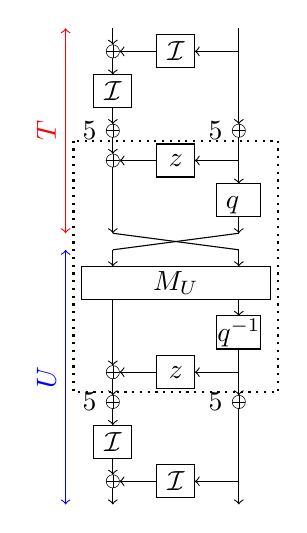
\begin{tikzpicture}[xscale=0.8, yscale=-0.42]
        \draw [->] (0,0) -- (0,0.5);
        \draw [very thin] (0,0.7) ellipse (0.105 and 0.2);
        \draw [very thin] (0,0.5) -- (0,0.9);
        \draw [very thin] (-0.105,0.7) -- (0.105,0.7);
        \draw (2,0) -- (2,0.7);
        \draw [->] (2,0.7) -- (1.3,0.7);
        \draw (0.7,0.2) rectangle (1.3,1.2) node[pos=0.5] {$\mathcal{I}$};
        \draw [->] (0.7,0.7) -- (0.105,0.7);
        \draw [->] (0,0.9) -- (0,1.4);
        \draw (-0.3,1.4) rectangle (0.3,2.4) node[pos=0.5] {$\mathcal{I}$};
        \draw [->] (0,2.4) -- (0,2.9);
        \draw [very thin] (0,3.1) ellipse (0.105 and 0.2);
        \draw [very thin] (0,2.9) -- (0,3.3);
        \draw [very thin] (-0.105,3.1) -- (0.105,3.1);
        \draw (-0.105,3.1) node[anchor=east] {5};
        \draw [->] (2,0.7) -- (2,2.9);
        \draw [very thin] (2,3.1) ellipse (0.105 and 0.2);
        \draw [very thin] (2,2.9) -- (2,3.3);
        \draw [very thin] (1.895,3.1) -- (2.105,3.1);
        \draw (1.895,3.1) node[anchor=east] {5};
        \draw [->] (0,3.3) -- (0,3.8);
        \draw [very thin] (0,4) ellipse (0.105 and 0.2);
        \draw [very thin] (0,3.8) -- (0,4.2);
        \draw [very thin] (-0.105,4) -- (0.105,4);
        \draw (2,3.3) -- (2,4);
        \draw [->] (2,4) -- (1.3,4);
        \draw (0.7,3.5) rectangle (1.3,4.5) node[pos=0.5] {$z$};
        \draw [->] (0.7,4) -- (0.105,4);
        \draw [->] (2,4) -- (2,4.7);
        \draw (1.65,4.7) rectangle (2.35,5.7) node[pos=0.5] {$q^{\color{white}1}$};
        \draw [->] (0,4.2) -- (0,6.2);
        \draw [->] (2,5.7) -- (2,6.2);
        \draw (0,6.2) -- (0,6.2);
        \draw (2,6.2) -- (2,6.2);
        \draw (2,6.2) -- (0,6.7);
        \draw (0,6.2) -- (2,6.7);
        \draw [->] (0,6.7) -- (0,7.2);
        \draw [->] (2,6.7) -- (2,7.2);
        \draw (-0.5,7.2) rectangle (2.5,8.2) node[pos=0.5] {$M_U$};
        \draw [->] (2,8.2) -- (2,8.7);
        \draw (1.65,8.7) rectangle (2.35,9.7) node[pos=0.5] {$q^{-1}$};
        \draw [->] (0,8.2) -- (0,10.2);
        \draw [very thin] (0,10.4) ellipse (0.105 and 0.2);
        \draw [very thin] (0,10.2) -- (0,10.6);
        \draw [very thin] (-0.105,10.4) -- (0.105,10.4);
        \draw (2,9.7) -- (2,10.4);
        \draw [->] (2,10.4) -- (1.3,10.4);
        \draw (0.7,9.9) rectangle (1.3,10.9) node[pos=0.5] {$z$};
        \draw [->] (0.7,10.4) -- (0.105,10.4);
        \draw [->] (0,10.6) -- (0,11.1);
        \draw [very thin] (0,11.3) ellipse (0.105 and 0.2);
        \draw [very thin] (0,11.1) -- (0,11.5);
        \draw [very thin] (-0.105,11.3) -- (0.105,11.3);
        \draw (-0.105,11.3) node[anchor=east] {5};
        \draw [->] (2,10.4) -- (2,11.1);
        \draw [very thin] (2,11.3) ellipse (0.105 and 0.2);
        \draw [very thin] (2,11.1) -- (2,11.5);
        \draw [very thin] (1.895,11.3) -- (2.105,11.3);
        \draw (1.895,11.3) node[anchor=east] {5};
        \draw [->] (0,11.5) -- (0,12);
        \draw (-0.3,12) rectangle (0.3,13) node[pos=0.5] {$\mathcal{I}$};
        \draw [->] (0,13) -- (0,13.5);
        \draw [very thin] (0,13.7) ellipse (0.105 and 0.2);
        \draw [very thin] (0,13.5) -- (0,13.9);
        \draw [very thin] (-0.105,13.7) -- (0.105,13.7);
        \draw (2,11.5) -- (2,13.7);
        \draw [->] (2,13.7) -- (1.3,13.7);
        \draw (0.7,13.2) rectangle (1.3,14.2) node[pos=0.5] {$\mathcal{I}$};
        \draw [->] (0.7,13.7) -- (0.105,13.7);
        \draw [->] (0,13.9) -- (0,14.4);
        \draw [->] (2,13.7) -- (2,14.4);
        \draw[color=red,<->] (-0.75,0) -- node[sloped,above]{$T$} (-0.75,6.2);
        \draw[color=blue,<->] (-0.75,6.7) -- node[sloped,above]{$U$} (-0.75,14.4);
        \draw [thick,dotted] (-0.625,3.4) rectangle (2.625,11);
    \end{tikzpicture}
    \FigDef{middle-affine-a}{Joining the decompositions of $T$ and $U$.}
  \end{subfigure}
  \hspace{0.2cm}
  \begin{subfigure}[t]{0.3\textwidth}
    \centering
    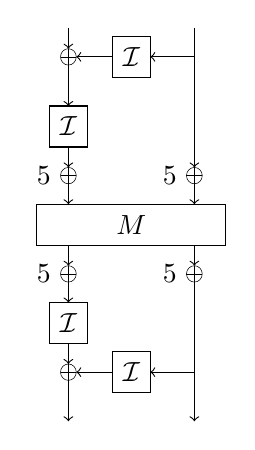
\begin{tikzpicture}[xscale=0.8, yscale=-0.52]
        \draw [->] (0,0) -- (0,0.5);
        \draw [very thin] (0,0.7) ellipse (0.125 and 0.2);
        \draw [very thin] (0,0.5) -- (0,0.9);
        \draw [very thin] (-0.125,0.7) -- (0.125,0.7);
        \draw (2,0) -- (2,0.7);
        \draw [->] (2,0.7) -- (1.3,0.7);
        \draw (0.7,0.2) rectangle (1.3,1.2) node[pos=0.5] {$\mathcal{I}$};
        \draw [->] (0.7,0.7) -- (0.125,0.7);
        \draw [->] (0,0.9) -- (0,1.9);
        \draw (-0.3,1.9) rectangle (0.3,2.9) node[pos=0.5] {$\mathcal{I}$};
        \draw [->] (0,2.9) -- (0,3.4);
        \draw [very thin] (0,3.6) ellipse (0.125 and 0.2);
        \draw [very thin] (0,3.4) -- (0,3.8);
        \draw [very thin] (-0.125,3.6) -- (0.125,3.6);
        \draw (-0.125,3.6) node[anchor=east] {5};
        \draw [->] (2,0.7) -- (2,3.4);
        \draw [very thin] (2,3.6) ellipse (0.125 and 0.2);
        \draw [very thin] (2,3.4) -- (2,3.8);
        \draw [very thin] (1.875,3.6) -- (2.125,3.6);
        \draw (1.875,3.6) node[anchor=east] {5};
        \draw [->] (0,3.8) -- (0,4.3);
        \draw [->] (2,3.8) -- (2,4.3);
        \draw (-0.5,4.3) rectangle (2.5,5.3) node[pos=0.5] {$M$};
        \draw [->] (0,5.3) -- (0,5.8);
        \draw [very thin] (0,6) ellipse (0.125 and 0.2);
        \draw [very thin] (0,5.8) -- (0,6.2);
        \draw [very thin] (-0.125,6) -- (0.125,6);
        \draw (-0.125,6) node[anchor=east] {5};
        \draw [->] (2,5.3) -- (2,5.8);
        \draw [very thin] (2,6) ellipse (0.125 and 0.2);
        \draw [very thin] (2,5.8) -- (2,6.2);
        \draw [very thin] (1.875,6) -- (2.125,6);
        \draw (1.875,6) node[anchor=east] {5};
        \draw [->] (0,6.2) -- (0,6.7);
        \draw (-0.3,6.7) rectangle (0.3,7.7) node[pos=0.5] {$\mathcal{I}$};
        \draw [->] (0,7.7) -- (0,8.2);
        \draw [very thin] (0,8.4) ellipse (0.125 and 0.2);
        \draw [very thin] (0,8.2) -- (0,8.6);
        \draw [very thin] (-0.125,8.4) -- (0.125,8.4);
        \draw (2,6.2) -- (2,8.4);
        \draw [->] (2,8.4) -- (1.3,8.4);
        \draw (0.7,7.9) rectangle (1.3,8.9) node[pos=0.5] {$\mathcal{I}$};
        \draw [->] (0.7,8.4) -- (0.125,8.4);
        \draw [->] (0,8.6) -- (0,9.6);
        \draw [->] (2,8.4) -- (2,9.6);
    \end{tikzpicture}
    \FigDef{middle-affine-b}{Merging linear layers.}
  \end{subfigure}
  \hspace{0.2cm}
  \begin{subfigure}[t]{0.3\textwidth}
    \centering
    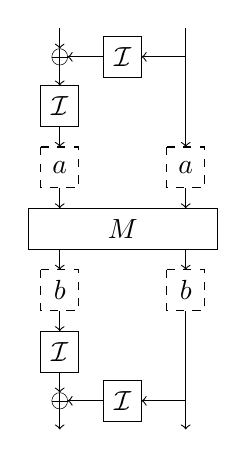
\begin{tikzpicture}[xscale=0.8, yscale=-0.52]
        \draw [->] (0,0) -- (0,0.5);
        \draw [very thin] (0,0.7) ellipse (0.125 and 0.2);
        \draw [very thin] (0,0.5) -- (0,0.9);
        \draw [very thin] (-0.125,0.7) -- (0.125,0.7);
        \draw (2,0) -- (2,0.7);
        \draw [->] (2,0.7) -- (1.3,0.7);
        \draw (0.7,0.2) rectangle (1.3,1.2) node[pos=0.5] {$\mathcal{I}$};
        \draw [->] (0.7,0.7) -- (0.125,0.7);
        \draw [->] (0,0.9) -- (0,1.4);
        \draw (-0.3,1.4) rectangle (0.3,2.4) node[pos=0.5] {$\mathcal{I}$};
        \draw [->] (0,2.4) -- (0,2.9);
        \draw [dashed] (-0.3,2.9) rectangle (0.3,3.9) node[pos=0.5] {$a$};
        \draw [->] (2,0.7) -- (2,2.9);
        \draw [dashed] (1.7,2.9) rectangle (2.3,3.9) node[pos=0.5] {$a$};
        \draw [->] (0,3.9) -- (0,4.4);
        \draw [->] (2,3.9) -- (2,4.4);
        \draw (-0.5,4.4) rectangle (2.5,5.4) node[pos=0.5] {$M$};
        \draw [->] (0,5.4) -- (0,5.9);
        \draw [dashed] (-0.3,5.9) rectangle (0.3,6.9) node[pos=0.5] {$b$};
        \draw [->] (2,5.4) -- (2,5.9);
        \draw [dashed] (1.7,5.9) rectangle (2.3,6.9) node[pos=0.5] {$b$};
        \draw [->] (0,6.9) -- (0,7.4);
        \draw (-0.3,7.4) rectangle (0.3,8.4) node[pos=0.5] {$\mathcal{I}$};
        \draw [->] (0,8.4) -- (0,8.9);
        \draw [very thin] (0,9.1) ellipse (0.125 and 0.2);
        \draw [very thin] (0,8.9) -- (0,9.3);
        \draw [very thin] (-0.125,9.1) -- (0.125,9.1);
        \draw (2,6.9) -- (2,9.1);
        \draw [->] (2,9.1) -- (1.3,9.1);
        \draw (0.7,8.6) rectangle (1.3,9.6) node[pos=0.5] {$\mathcal{I}$};
        \draw [->] (0.7,9.1) -- (0.125,9.1);
        \draw [->] (0,9.3) -- (0,9.8);
        \draw [->] (2,9.1) -- (2,9.8);
    \end{tikzpicture}
    \FigDef{middle-affine-c}{Allowed transformations.}
  \end{subfigure}
  \FigDef{middle-affine}{Simplifying the middle affine layer. The linear mappings in the dotted area in \FigRef{middle-affine-a} form the linear layer $M$.}
\end{figure}